\documentclass[tikz,border=10pt]{standalone}
\usepackage{tikz}
\usetikzlibrary{arrows.meta,calc}

\begin{document}
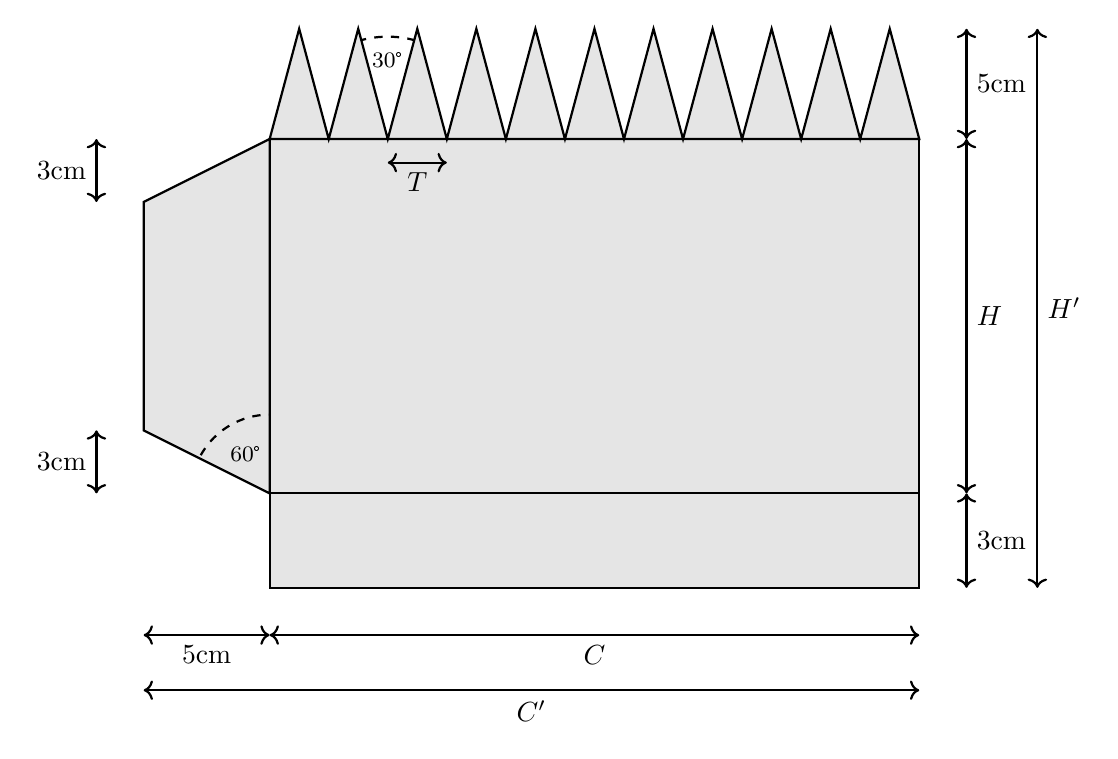
\begin{tikzpicture}[line width=0.8pt]

% ---------- Parameters of the drawing ----------
% Dimensions of the drawing
\def\CylHeight{4.5}          % Height H of the cylinder
\def\LowerFlapHeight{1.2}          % Height of the lower flap
\def\nTeeth{11}       % Total number of teeth
\def\ToothHeight{1.4}           % Height of a tooth
\def\ToothWidth{0.75}  % Width of a tooth
\def\LeftFlapWidth{1.6}          % Width of the left flap
\def\LeftFlapHeightShorten{0.8}  % Amount by which the height of the left flap is shortened relative to the height of the cylinder

% Distance to dimensioning labels
\def\LowerDimensioningDistanceShort{0.6} % Vertical distance between the drawing and the dimensioning on the bottom
\def\LowerDimensioningDistanceLong{1.3}
\def\RightDimensioningDistanceShort{0.6} % Horizontal distance between the drawing and the dimensioning on the right
\def\RightDimensioningDistanceLong{1.5}
\def\UpperDimensioningDistance{0.3}
\def\LeftDimensioningDistance{0.6}

% Angle label on the left flap
\def\LeftFlapAngleRadius{1}
\def\LeftFlapAngleLabelXShift{-0.3}
\def\LeftFlapAngleLabelYShift{0.5}

% Angle label on the teeth
\def\ToothAngleRadius{1.3}
\def\ToothAngleLabelYShift{1}

% ---------- Derived parameters of the drawing ----------
\pgfmathsetmacro{\RectangleWidth}{\nTeeth*\ToothWidth} % Circumference C of the head of the PhD student
\pgfmathsetmacro{\LeftFlapAngle}{atan(\LeftFlapWidth / \LeftFlapHeightShorten)}

% ---------- Labels of the drawing ----------
\def\ToothWidthLabel{$ T $}
\def\LeftFlapWidthLabel{5cm}
\def\RectangleWidthLabel{$ C $}
\def\TotalWidthLabel{$ C' $};

\def\ToothHeightLabel{5cm}
\def\CylHeightLabel{$ H $}
\def\LowerFlapHeightLabel{3cm}
\def\TotalHeightLabel{$ H' $}
\def\LeftFlapHeightShortenLabel{3cm}

\def\LeftFlapAngleLabel{60°}
\def\ToothAngleLabel{30°}

% ---------- Colours ----------
\colorlet{fillcolor}{black!10}
\colorlet{helplinecolor}{gray}


% (0,0) coordinate = upper left corner of rectangle

% ---------- Basic rectangle ----------
\draw[fill=fillcolor] (0,0) rectangle (\RectangleWidth,-\CylHeight);

% ---------- Lower flap ----------
\draw[fill=fillcolor] (0,-\CylHeight) rectangle (\RectangleWidth, -\CylHeight-\LowerFlapHeight);
% Trennlinie zwischen H-Bereich und 3cm-Streifen
\draw (0,-\CylHeight) -- (\RectangleWidth,-\CylHeight);

% ---------- Left flap + angle ----------
\begin{scope}
	\draw[fill=fillcolor] (-\LeftFlapWidth,-\LeftFlapHeightShorten) -- (0,0) -- (0,-\CylHeight) -- ++(-\LeftFlapWidth, \LeftFlapHeightShorten) -- cycle;
	% Draw the arc around the desired angle by clipping a full circle to the path of the left flap
	\path[clip] (-\LeftFlapWidth,-\LeftFlapHeightShorten) -- (0,0) -- (0,-\CylHeight) -- ++(-\LeftFlapWidth, \LeftFlapHeightShorten) -- cycle;
	\draw[dashed] (0,-\CylHeight) circle[radius=\LeftFlapAngleRadius];
	\node[font=\footnotesize] at (\LeftFlapAngleLabelXShift, -\CylHeight+\LeftFlapAngleLabelYShift){\LeftFlapAngleLabel};
\end{scope}


% ---------- Teeth on top ----------
\draw[fill=fillcolor]
	(0,0)
	\foreach \i in {1,...,\nTeeth} {
	  -- ++(\ToothWidth/2,\ToothHeight) -- ++(\ToothWidth/2,-\ToothHeight)
	}
	-- cycle;

% ---------- Dimensioning: Width ----------
\begin{scope}
	% Left flap-
	\draw[<->] (0,-\CylHeight-\LowerFlapHeight-\LowerDimensioningDistanceShort) -- ++(-\LeftFlapWidth,0) node[midway,below]{\LeftFlapWidthLabel};
	% Rectangle
	\draw[<->] (0,-\CylHeight-\LowerFlapHeight-\LowerDimensioningDistanceShort) -- ++(\RectangleWidth,0) node[midway,below]{\RectangleWidthLabel};
	% Total width
	\draw[<->] (-\LeftFlapWidth,-\CylHeight-\LowerFlapHeight-\LowerDimensioningDistanceLong) -- ++(\LeftFlapWidth+\RectangleWidth, 0) node[midway,below]{\TotalWidthLabel};
\end{scope}

% ---------- Dimensioning: Height, right ----------
\begin{scope}
	% Teeth
	\draw[<->] (\RectangleWidth+\RightDimensioningDistanceShort,0)-- ++(0,\ToothHeight) node[midway,right]{\ToothHeightLabel};
	% Cylinder
	\draw[<->] (\RectangleWidth+\RightDimensioningDistanceShort,0) -- ++(0,-\CylHeight) node[midway,right]{\CylHeightLabel};
	% Lower flap
	\draw[<->] (\RectangleWidth+\RightDimensioningDistanceShort,-\CylHeight) -- ++(0,-\LowerFlapHeight) node[midway,right]{\LowerFlapHeightLabel};
	% Total
	\draw[<->] (\RectangleWidth+\RightDimensioningDistanceLong,\ToothHeight)-- ++(0,-\ToothHeight-\CylHeight-\LowerFlapHeight) node[midway,right]{\TotalHeightLabel};
\end{scope}

% ---------- Dimensioning: Height, left ----------
\foreach \y\sign in {0/-, -\CylHeight/+}{
	\draw[<->] (-\LeftFlapWidth-\LeftDimensioningDistance, \y) -- ++(0, \sign\LeftFlapHeightShorten) node[midway,left]{\LeftFlapHeightShortenLabel};
}

% ---------- Dimensioning: Teeth ----------
\draw[<->] (2*\ToothWidth, -\UpperDimensioningDistance) -- ++(\ToothWidth,0) node[midway,below]{\ToothWidthLabel};

% ---------- Angle on teeth ----------
\begin{scope}
	\coordinate (base) at (2*\ToothWidth,0);
	\path[clip] (base) -- +(-\ToothWidth/2, \ToothHeight) -- +(\ToothWidth/2, \ToothHeight) -- cycle;
	\draw[dashed] (base) circle[radius=\ToothAngleRadius];
	
	\node[font=\footnotesize] at ($ (base) + (0,\ToothAngleLabelYShift) $){\ToothAngleLabel};
\end{scope}


\end{tikzpicture}
\end{document}
